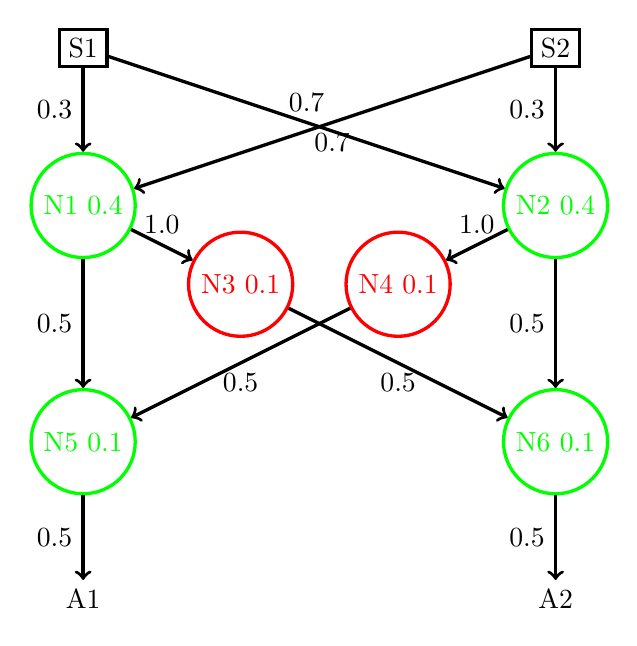
\begin{tikzpicture}[scale=0.5]
 \tikzset{directed/.style={->}} 
  \node[] (A1) at (0,0) {A1};
  \node[] (A2) at (12,0) {A2};
  \node[draw, circle, very thick, color=green] (N1) at (0,10) {N1 0.4};
  \node[draw, circle, very thick, color=green] (N2) at (12,10) {N2 0.4};
  \node[draw, circle, very thick, color=red] (N3) at (4,8) {N3 0.1};
  \node[draw, circle, very thick, color=red] (N4) at (8,8) {N4 0.1};
  \node[draw, circle, very thick, color=green] (N5) at (0,4) {N5 0.1};
  \node[draw, circle, very thick, color=green] (N6) at (12,4) {N6 0.1};
  \node[draw, very thick] (S1) at (0,14) {S1};
  \node[draw, very thick] (S2) at (12,14) {S2};
  \draw[very thick, directed] (S1) -- node[left] {0.3}(N1);
  \draw[very thick, directed] (S1) -- node[above] {0.7}(N2);
  \draw[very thick, directed] (S2) -- node[below] {0.7}(N1);
  \draw[very thick, directed] (S2) -- node[left] {0.3}(N2);
  \draw[very thick, directed] (N1) -- node[above] {1.0}(N3);
  \draw[very thick, directed] (N2) -- node[above] {1.0}(N4);
  \draw[very thick, directed] (N3) -- node[below] {0.5}(N6);
  \draw[very thick, directed] (N4) -- node[below] {0.5}(N5);
  \draw[very thick, directed] (N1) -- node[left] {0.5}(N5);
  \draw[very thick, directed] (N2) -- node[left] {0.5}(N6);
  \draw[very thick, directed] (N5) -- node[left] {0.5}(A1);
  \draw[very thick, directed] (N6) -- node[left] {0.5}(A2);
\end{tikzpicture}
